\def\year{2015}
\def\thetitle{An Ensemble Method to Produce High-Quality Word Embeddings}

% Update this when our score changes.
\def\scoreRW{.604}   % score on RW [all]
\def\scoreMEN{.867}  % score on MEN-3000 [test]
\def\yes{\textbullet}

\documentclass[11pt,letterpaper]{article}
% Packages required by the paper format
\usepackage{naaclhlt2016}
\usepackage{times}
\usepackage{latexsym}
\usepackage{amsmath}
\usepackage{booktabs}

%\naaclfinalcopy % Uncomment this line for the final submission
\def\naaclpaperid{***} %  Enter the naacl Paper ID here

% Packages we need
\usepackage{pgfplots}
\pgfplotsset{compat=1.9}
\usepackage{CJKutf8}
\usepackage{url}
\usepackage{graphicx}
\bibliographystyle{naaclhlt2016}

\title{\thetitle}
\author{Robert Speer\\
    Luminoso Technologies, Inc.\\
    675 Massachusetts Ave.\\
    Cambridge, MA 02139\\
    \texttt{rspeer@luminoso.com}
\And
    Joshua Chin\\
    Union College\\
    807 Union St.\\
    Schenectady, NY 12308\\
    \texttt{joshuarchin@gmail.com}
}

\date{}

\begin{document}

\maketitle
\begin{abstract}

A currently successful approach to computational semantics is to represent
words as embeddings in a machine-learned vector space. We
present an ensemble method that combines embeddings produced by GloVe
\cite{pennington2014glove} and word2vec \cite{mikolov2013word2vec} with
structured knowledge from the semantic network ConceptNet 5
\cite{speer2012conceptnet}, merging their
information into a common representation with a large, multilingual vocabulary.
The embeddings it produces achieve state-of-the-art performance on many word
similarity evaluations. Its score of $\rho = \scoreRW{}$ on an evaluation of
rare words \cite{luong2013rw} is 17\% higher than the previous best known
system.

\end{abstract}

\section{Introduction}

Vector space models are an effective way to express the meanings of
natural-language terms in a computational system. These models are created
using machine-learning techniques that represent words or phrases as
vectors in a high dimensional space, such that the cosine similarity of any two
terms corresponds to their semantic similarity.

These vectors, referred to as
the {\em embeddings} of the terms in the vector space, can be compared directly
to measure the similarity of two terms (as the cosine similarity of their
respective vectors), and can also be used as an input to further steps of
machine learning. When algorithms expect dense vectors as input, embeddings
provide a representation that is both more compact and more informative than the
``one-hot'' representation in which every term in the vocabulary gets its own
dimension.

This kind of vector space has been used in applications such as search, topic
detection, and text classification, dating back to the introduction of latent
semantic analysis \cite{deerwester1990indexing}.  In recent years, there has
been a surge of interest in natural-language embeddings, as machine-learning
techniques such as \newcite{mikolov2013word2vec}'s word2vec and
\newcite{pennington2014glove}'s GloVe have begun to show dramatic improvements.
Word embeddings are often suggested as an initialization for more complex
methods, such as the sentence encodings of \newcite{kiras2015skip}.

\newcite{faruqui2015retrofitting} introduced a technique
known as ``retrofitting'', which combines embeddings learned from the
distributional semantics of unstructured text with a source of structured
connections between words. The combined embedding achieves performance on
word-similarity evaluations superior to either source individually.

Here, we build on the retrofitting process to produce a high-quality space of
word embeddings. We extend existing techniques in the following ways:

\begin{itemize}
\item We include ConceptNet, a Linked Open Data semantic network that expresses
many kinds of relationships between words in many languages, as a source of
structured connections between words.
\item We modify the retrofitting algorithm, making it not depend on the row
order of its input matrix, and allowing it to propagate over the union of the
vocabularies. We call this procedure ``expanded retrofitting''.
\item We align English terms from different sources using a lemmatizer and a
heuristic for merging together multiple term vectors.
\item We fill gaps when aligning the two distributional-semantics sources
(GloVe and word2vec) using a locally linear interpolation.
\item We re-scale the distributional-semantics features using $L_1$ normalization.
\end{itemize}

When we use this process to combine word2vec, GloVe, and ConceptNet, this
process produces a space of term embeddings
that achieves state-of-the-art performance on word-similarity
evaluations\footnote{Some methods and evaluations \cite{agirre2009study}
distinguish word similarity from word
{\em relatedness}. ``Coffee'' and ``mug'', for example, are quite related,
but not actually similar because coffee is not {\em like} a mug. In this paper,
however, we conflate similarity and relatedness into the same metric, as most
evaluations do.}
over both common and rare words.


\subsection{Related work}

% TODO: talk about Agirre's observation of distributional vs. structured data
% TODO: cite Turney 2010 survey
% TODO: cite Levy 2015
% TODO: talk about Bian and word senses

\section{Knowledge sources}

\subsection{ConceptNet and PPDB}
ConceptNet \cite{speer2012conceptnet} is a semantic network of terms
connected by labeled relations. Its terms are words or multiple-word phrases
in a variety of natural languages. For continuity with previous work,
these terms are often referred to as {\em concepts}.

ConceptNet originated as a machine-parsed version of the early crowd-sourcing
project called Open Mind Common Sense (OMCS) \cite{singh2002omcs}, and has expanded
to include several other data sources, both crowd-sourced and expert-created,
by unifying their vocabularies into a single representation. ConceptNet now includes
representations of WordNet \cite{miller1998wordnet}, Wiktionary \cite{wiktionary2014en},
and JMDict \cite{breen2004jmdict}, as well as data from ``games with a purpose'' in
multiple languages \cite{vonahn2006verbosity} \cite{kuo2009petgame}
\cite{nakahara2011nadya}. We choose not to include ConceptNet's alignment to DBPedia
here, as DBPedia focuses on relations between specific named entities, which do not help
with general word similarity.\footnote{
    Given different goals -- such as achieving a high score on
    \newcite{mikolov2013word2vec}'s analogy evaluation that tests for
    implicit relations such as ``{\em A} is the CEO of company {\em B}'' --
    including an appropriate representation of DBPedia would of course be helpful.
}

PPDB \cite{ganitkevitch2013ppdb} is another resource that is useful for
learning about word similarity, providing different information from
ConceptNet. It lists pairs of words that are translated to the same word in parallel
corpora, particularly in documents of the European Parliament. PPDB is used
as an external knowledge source by \newcite{faruqui2015retrofitting}, so
we evaluate the effect of adding it to our ensemble as well.

\subsection{word2vec and GloVe}

word2vec and GloVe are two current systems that learn vector representations
of words according to their distributional semantics. Given a large text corpus,
they produce vectors representing similarities in how the words co-occur with
other words.

\newcite{mikolov2013word2vec} described a system of distributional word
embeddings called Skip-Grams with Negative Sampling (SGNS), which is more
popularly known by the name of its software implementation, {\em word2vec}.
(The {\em word2vec} software also implements another representation, Continuous
Bag-of-Words or CBOW, which is less often used for word similarity.)

In SGNS, a neural network with one hidden layer is trained to recognize words
that are likely to appear near each other. Its goal is to output a high value
when given examples of co-occurrences that appear in the data, and a low value
for negative examples where one word is replaced by a random word. The loss
function is weighted by the frequencies of the words involved and the distance
between them in the data. The word2vec
software\footnote{\url{https://code.google.com/p/word2vec/}} comes with SGNS
embeddings of text from Google News.

GloVe \cite{pennington2014glove} is an unsupervised learning algorithm that
learns a set of word embeddings such that the dot product of two words'
embeddings is approximately equal to the logarithm of their co-occurrence count.
The algorithm operates on a global word-word co-occurrence matrix, and
solves an optimization problem to learn a vector for each word, a separate
vector for each context (although the contexts are also words), and a bias
value for each word and each context. Only the word vectors are used for
computing similarity.

The embeddings that GloVe learns from data sources such as the Common
Crawl\footnote{\url{http://commoncrawl.org/}} are distributed on the GloVe web
page\footnote{\url{http://nlp.stanford.edu/projects/glove/}}. Here we evaluate
two downloadable sets of GloVe 1.2 embeddings, built from 42 billion and 840
billion tokens of the Common Crawl, respectively.

% NOTE: we may need to squish the next two paragraphs
There is some debate about whether GloVe or word2vec is better at representing
word meanings in general. GloVe is presented by \newcite{pennington2014glove}
as performing better than word2vec on word similarity tasks, but
\newcite{levy2015embeddings} finds that word2vec performs better with an
optimized setting of hyperparameters than GloVe does, when retrained with a
particular corpus.

In this paper, we focus only on the downloadable sets of term embeddings that
the GloVe and word2vec projects provide, not on re-running them with tuned
hyperparameters. Using this data makes it possible to reproduce their results
and compare directly to them, even when their preferred input data is not
publically available. We find that we can get very good results derived from
the downloadable embeddings, and that GloVe's downloadable embeddings outperform
word2vec's in this case, but a combination of them can perform even better.

\section{Methods}

\begin{figure}
\centering
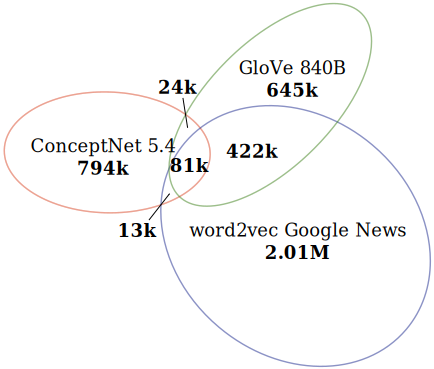
\includegraphics[width=2.5in]{areas.pdf}
\caption{
    A proportional-area diagram showing the overlap of vocabularies among
    ConceptNet and the available embeddings for word2vec and GloVe.
}
\label{vocabulary-overlap}
\end{figure}

\newcite{faruqui2015retrofitting} introduced the ``retrofitting'' procedure,
which adjusts dense matrices of embeddings (such as the GloVe output) to take
into account external knowledge from a sparse semantic network. They tried
various sources of external knowledge, and the one that was most helpful to
GloVe was PPDB.  We found using ConceptNet to be more effective, and that
further marginal improvements could be achieved on some evaluations by
combining ConceptNet and PPDB.

% FIXME: does this paragraph go somewhere else?
Our goal is to create a 300-dimensional vector space that represents terms based
on a combination of GloVe and word2vec's downloadable embeddings, and structured
data from ConceptNet and PPDB. The resulting vector space allows information to
be shared among these various representations, including words that were not in
the vocabulary of the original representations. This includes low-frequency words
and even words that are not in English.

\subsection{Standardizing Text}

As \newcite{levy2015embeddings} notes,
``[\ldots] much of the performance gains of word embeddings are due to certain
system design choices and hyperparameter optimizations, rather than the
embedding algorithms themselves.'' While it is presented as a negative result,
this simply emphasizes the importance of these system design choices.

Indeed, we have found that choices about how to handle terms and their
embeddings have a significant impact on evaluation results. One of these choices
involves how to pre-process words and phrases before looking them up, and
another involves the scale of the various features in the embeddings.


\subsubsection{Transforming and Aligning Vocabularies}

Different representations apply
different pre-processing steps, placing strings in different equivalence
classes. We can only properly combine these resources if these string
representations are comparable to each other.

% TODO: check this list

Pre-processing steps that various resources apply include: tokenizing text to
separate words from punctuation (which all inputs except GloVe 840B do),
joining multi-word phrases with underscores (ConceptNet and word2vec), removing
a small list of stopwords from multi-word phrases (ConceptNet only), folding the text to lowercase
(ConceptNet and GloVe 42B), replacing multiple digits with the character {\tt
\#} (word2vec only), and lemmatizing English words to their root form using a
modification of WordNet's Morphy algorithm (ConceptNet only).

We adapt a text pre-processing function from ConceptNet to apply a combination
of all of these processes, yielding a set of standardized, language-tagged
labels. As an example, the text ``Giving an example'' becomes the standardized
form {\tt /c/en/give\_example}. Applying this combined pre-processing function
to all labels increases the alignment of the various resources while reducing
the size of the combined vocabulary.

Because the transformations are many-to-one, this has the effect that a single
transformed term can become associated with multiple embeddings in a single
vector space. We considered a few options for dealing with these merged terms,
such as keeping only the highest-frequency term, averaging the vectors together,
or taking a weighted average based on their word frequency.

We found in preliminary evaluations that the weighted average was the best
approach. The multiple rows contain valuable data that should not simply be
discarded, but lower-frequency rows tend to have lower-quality data.

When using pre-trained vectors, it is often the case that intermediate
computations that produced these vectors (such as word frequencies) are not
available. What we do instead is to infer approximate word frequencies from
the fact that both GloVe and word2vec output their vocabularies in descending
order of frequency. We approximate the frequency distribution by assuming that
the tokens are distributed according to Zipf's law \cite{zipf1949human}: the
$n$th token in rank order has a frequency proportional to $1/n$. We use these
proportions in the weighted average when combining multiple embeddings.

This process alone is a benefit on word-similarity evaluations, even without
combining any resources. For example, the Rare Words (RW) dataset
\cite{luong2013rw} tends to encounter terms that are poorly represented or
out-of-vocabulary in most word embeddings.  Lemmatizing them before looking
them up, and combining them with more frequently observed representations,
improves the evaluation results on these words, even though the process
loses the ability to distinguish some word forms. The raw GloVe 840B data gets
a Spearman correlation of $\rho = .146$ on the RW dataset, which increases to
$\rho = .494$ when its embeddings are standardized and combined in this way.

Figure~\ref{vocabulary-overlap} shows the size of the vocabularies of
ConceptNet, GloVe, and word2vec after this transformation, and the sizes of
the overlaps among them, using a proportional-area Venn diagram produced using
{\em eulerAPE} \cite{micallef2014euler}.

\subsubsection{Feature Normalization}

As briefly mentioned by \newcite{pennington2014glove}, $L_2$ normalization of
the columns (that is, the 300 features) of the GloVe matrix provides a notable
increase in performance. One effect of normalization is to increase the weight
of distinguishing features and reduce the impact of noisy features.  Features
are more distinguishing for the purpose of cosine similarity when they contain
a few large values and many small ones.

We find that $L_1$ normalization of GloVe performs even better than $L_2$
normalization. $L_1$ causes occasional large values to have a smaller impact on the norm
than $L_2$ normalization. When a learning method such as GloVe has provided
highly selective features, $L_1$ normalization allows us to use them more effectively
in measuring similarity.


\subsection{Retrofitting}

% TODO: restate less about how retrofitting works?

Retrofitting \cite{faruqui2015retrofitting} is a process of combining existing
word vectors with a semantic lexicon. While the original formulation expresses
the problem in terms of updates that propagate over a set of edges, we have
found it more convenient to express it and implement it in terms of an update
to a matrix.

The inputs to retrofitting are an initial dense matrix of term embeddings,
$W^0$, and a sparse matrix of known semantic relationships, $S$. Let the size
of the complete vocabulary be $m$ and the dimensionality of the embeddings be $n$.
$W^0$ is an $m \times n$ matrix containing the known term embeddings, with
rows of all zeroes for terms that are outside the vocabulary of the original embeddings.
$S$ is an $n \times n$ matrix containing positive weighted values for terms that
are known to be semantically related, 1 on the diagonal relating each term to
itself, and 0 otherwise.

Retrofitting on a matrix $W$ (whose rows are indicated by $w_i$) yields a final
matrix $W'$ (with rows indicated by $w'_i$) that minimizes

\begin{small}
$$
\Psi \left( W' \right) = \sum_{i=1}^v \left[
  \alpha_i \left\|  w'_i - w_i \right\| ^ 2
  + \sum_{j=1}^v S_{ij} \left\| w'_i - w'_j \right\| ^ 2
\right]
$$
\end{small}

where $\alpha$ is a vector that indicates the weight of a term in the original
vector space. For our purposes, we let $\alpha_i$ be 1 when word $i$ is in the
original embeddings' vocabulary, and 0 when it only appears in the semantic
network. (This neutralizes the effect of the all-zero rows in $W^0$.) We can
also represent these weights as a diagonal matrix $A$, where $A_{ii} =
\alpha_i$, allowing us to multiply matrices by it row-wise.

Similarly to the original formulation of retrofitting, $\Psi$ can be optimized
by a simple iterative updating method. We repeatedly update $W$ with:

$$
W^{k+1} = \mathrm{normalize}\left( \left( S W^k + W^0 A \right)\left( 1 + A \right)^{-1} \right)
$$

where $A$ is a matrix whose diagonal is the weight vector $\alpha$. The {\em normalize}
function applies $L_2$ normalization to each non-zero row of its argument, ensuring
that terms are always represented by unit vectors that can be used directly in
cosine similarity.

\subsection{ConceptNet as an Association Matrix}

In order to apply the expanded retrofitting method, we need to consider the data in
ConceptNet as a sparse, symmetric matrix of associations between terms. What
ConceptNet provides is more complex than that, as it connects terms with a
variety of not-necessarily-symmetric, labeled relations.

\newcite{havasi2010color} introduced a vector space embedding of ConceptNet,
``spectral association'', that disregarded the relation labels for the purpose
of measuring the relatedness of terms. Previous embeddings of ConceptNet, such
as that of \newcite{speer2008analogyspace}, preserved the relations but were
suited mostly for direct similarity and inference, not for relatedness. Because
most evaluation data for word similarity is also evaluating relatedness, unless
there has been a specific effort to separate them \cite{agirre2009similarity},
we erase the labels as in spectral association.

Negated relations and antonym relations, such as the relations expressed by
``a person does not have a tail'' and ``hot is the opposite of cold'', are
typically handled specially; a detail of spectral association is that negated
relations were assigned negative values in the matrix. Intuitively, negated
relations between two terms should not increase their relatedness. Perhaps
these relations should in fact decrease relatedness -- while ``hot'' and
``cold'' are similar in many ways, people providing judgments of relatedness
are likely to consider them less related because of the obvious contrast
between them.

However, association matrices are better behaved when they contain no negative
entries. Saying that vector $A$ should be a bit less related to vector
$B$ is very different from saying that it should be related to $-B$.
In our method, we simply omit all instances of negative and antonym
relations in ConceptNet.

Each remaining assertion in ConceptNet corresponds to two entries in a sparse
association matrix $S$.  ConceptNet assigns a confidence score, or weight, to
each assertion.  These weights are not entirely comparable between the data
sources that comprise ConceptNet, so we re-scaled them so that the average
weight of each different data source is 1.

An assertion that relates term $i$ to term $j$ with adjusted weight $w$ will
contribute $w$ to the values of $S_{ij}$ and $S_{ji}$. If another assertion
relates the same terms with a different relation, it will add to that value.
This constructs a symmetric matrix $S$, but the matrix we actually use in
retrofitting is the asymmetric $S'$, whose rows have been $L_1$-normalized to
prevent high-frequency concepts from overwhelming the results.

Due to the structure of ConceptNet, there exists a large fringe of terms that are
poorly connected to other nodes. To make the sparse matrix and the size of the
overall vocabulary more manageable, we filter ConceptNet when building its
association matrix: we exclude all terms that appear fewer than 3 times, English
terms that appear fewer than 4 times, and terms with more than 3 words in them.

\subsection{Locally Linear Alignment}

In order to use both word2vec and GloVe at the same time, we need to align their
partially-overlapping vocabularies and merge their features. This is
straightforward to do on the terms that are shared between the two vocabularies,
but we would rather not lose the other terms, if we can later benefit from
learning more about those terms from ConceptNet.

Before merging features, we need to compute GloVe representations for terms
represented in word2vec but not GloVe, and vice versa. The way we do this
is inspired by \newcite{zhao2015learning}, who infer translations between
languages of unknown phrases using a locally-linear projection of known
translations of similar phrases. Instead of known translations, we have the
terms that overlap between word2vec and GloVe. Given a non-overlapping term,
we calculate its vector as the average of the vectors of the nearest
overlapping terms, weighted by their cosine similarity.

To combine the features of word2vec and GloVe, we first concatenate their
vectors into 600-dimensional vectors, then make the result more compact and
less redundant by reducing them back to 300 dimensions using a truncated SVD.
We factor the 600-dimensional matrix $A$ as $A \approx U \Sigma V^T$, keeping
only the 300 largest eigenvalues, then compute the new 300-dimensional joint
features as $U \Sigma^{1/2}$.

\section{Evaluation}

\subsection{Word Similarity Datasets}

We evaluate our model's performance at identifying similar words using a
variety of word-similarity gold standards:

\begin{itemize}
\item MEN-3000 \cite{bruni2014men}, crowd-sourced similarity judgments for 3000
    word pairs.
\item The Stanford Rare Words (RW) dataset \cite{luong2013rw}, crowd-sourced
    similarity judgments for 2034 word pairs, with a bias toward uncommon words.
\item WordSim-353 \cite{finkelstein2001ws}, a widely-used corpus of similarity
    judgments for 353 word pairs.
\item RG-65 \cite{rubenstein1965rg}, a classic corpus of similarity judgments
    for 65 word pairs, which has additionally been translated into German
    \cite{gurevych2005german} and French \cite{joubarne2011french}.
\end{itemize}

In striving to maximize an evaluation metric, it is important to hold out some
data, to avoid overfitting to the data by modifying the algorithm and its
parameters.

MEN-3000 comes with a development/test split, where 1000 of the 3000 word pairs
are held out for testing. We applied a similar split to RW, setting aside a
sample of $1/3$ of its word pairs for testing.\footnote{
    We set aside every third row, starting from row 3, using the Unix command
    {\tt split -un r/3/3 rw.txt}. Similarly, we split on {\tt r/1/3} and
    {\tt r/2/3} and concatenated the results to get the remaining evaluation
    data.
} We did not apply a split to WordSim-353, as it is already much smaller than
the others.

Neither of the held-out test sets were used in our evaluations during
development; they were only run with the final code and parameters. While
Table~\ref{eval-bigtable} shows our correlation with only the test data on
these evaluations, Table~\ref{eval-dev-test} compares our performance on
development and test data.

\subsection{Results}

\begin{table}[ht]
\centering
\footnotesize
\begin{tabular}{llllll|rrr}
\toprule
\multicolumn{6}{c|}{Ensemble components} & \multicolumn{3}{c}{Evaluations} \\
\bf CN&\bf PP&\bf St&\bf W& \bf G& $L_1$  & \bf RW  & \bf MEN & \bf  WS \\
\midrule
     &      &      &      & g    &        &    .448 &    .816 &    .759 \\  % glove.42B.300d.l2.raw.evaluation
     &      &      &      & g    & $L_1$  &    .457 &    .820 &    .766 \\  % glove.42B.300d.l1.raw.evaluation
     &      &      &      & G    &        &    .146 &    .787 &    .671 \\  % glove12.840B.300d.l2.raw.evaluation
     &      &      &      & G    & $L_1$  &    .148 &    .789 &    .676 \\  % glove12.840B.300d.l1.raw.evaluation
     &      &      & W    &      &        &    .371 &    .732 &    .624 \\  % w2v-google-news.none.raw.evaluation
     &      &      & W    &      & $L_1$  &    .374 &    .732 &    .622 \\  % w2v-google-news.l1.raw.evaluation
\midrule
     &      & St   &      & g    &        &    .492 &    .815 &    .765 \\  % glove.42B.300d.l2.standardized.evaluation
     &      & St   &      & g    & $L_1$  &    .513 &    .834 &    .794 \\  % glove.42B.300d.l1.standardized.evaluation
     &      & St   &      & G    &        &    .494 &    .814 &    .763 \\  % glove12.840B.300d.l2.standardized.evaluation
     &      & St   &      & G    & $L_1$  &    .513 &    .840 &    .798 \\  % glove12.840B.300d.l1.standardized.evaluation
     &      & St   & W    &      &        &    .453 &    .778 &    .731 \\  % w2v-google-news.none.standardized.evaluation
     &      & St   & W    &      & $L_1$  &    .452 &    .777 &    .732 \\  % w2v-google-news.l1.standardized.evaluation
     &      & St   & W    & G    & $L_1$  &    .539 &    .841 &    .796 \\  % combo.l1.standardized.evaluation
\midrule
     & PP   & St   &      & G    & $L_1$  &    .565 &    .852 &    .806 \\  % glove12.840B.300d.l1.standardized.ppdb-xl-lexical-standardized.evaluation
     & PP   & St   & W    &      & $L_1$  &    .481 &    .800 &    .750 \\  % w2v-google-news.l1.standardized.ppdb-xl-lexical-standardized.evaluation
     & PP   & St   & W    & G    & $L_1$  &    .558 &    .850 &    .806 \\  % combo.l1.standardized.ppdb-xl-lexical-standardized.evaluation
CN   &      & St   &      & G    & $L_1$  &    .571 &    .856 &    .818 \\  % glove12.840B.300d.l1.standardized.conceptnet5.evaluation
CN   &      & St   & W    &      & $L_1$  &    .542 &    .813 &    .771 \\  % w2v-google-news.l1.standardized.conceptnet5.evaluation
CN   &      & St   & W    & G    & $L_1$  &    .611 &\bf .868 &\bf .821 \\  % combo.l1.standardized.conceptnet5.evaluation
CN   & PP   & St   &      & G    & $L_1$  &    .584 &    .860 &    .818 \\  % glove12.840B.300d.l1.standardized.cnet-ppdb-combined.evaluation
CN   & PP   & St   & W    &      & $L_1$  &    .543 &    .812 &    .775 \\  % w2v-google-news.l1.standardized.cnet-ppdb-combined.evaluation
CN   & PP   & St   & W    & G    & $L_1$  &\bf .613 &    .867 &\bf .821 \\  % combo.l1.standardized.cnet-ppdb-combined.evaluation
\bottomrule
\end{tabular}

\caption{
    Word-similarity results as various components of the ensemble are enabled.
    The results are the Spearman rank correlation ($\rho$) with the held-out
    test sets of RW and MEN-3000 and with WordSim-353.
    The components are: {\bf CN} = ConceptNet 5.4,
    {\bf PP} = PPDB-xl, {\bf St} = standardized and lemmatized terms,
    {\bf W} = word2vec vectors from SGNS on Google News, {\bf g} = GloVe 42B vectors,
    {\bf G} = GloVe 1.2 840B vectors, {\bf $L_1$} = $L_1$-normalized features.
}
\label{eval-bigtable}
\end{table}


\begin{table}[t]
\centering
\footnotesize
\begin{tabular}{l|rrr}
\toprule
Method                        & RW [all]  &      MEN  & WS \\
\midrule
word2vec SGNS (Levy)          &     .470  &     .774  & .733* \\
word2vec SGNS (ours)          &     .476  &     .778  & .731  \\
GloVe (Pennington)            &     .448  &     .816  & .759  \\
GloVe (ours)                  &     .528  &     .840  & .798  \\
SVD (Levy)                    &     .514  &     .778  & .736* \\
Retrofitting (Faruqui)        &      ---  &     .796  & .741  \\
Our ensemble                  & \bf .604  & \bf .868  & \bf .821 \\
\bottomrule
\end{tabular}

\caption{
    Comparison between our ensemble word embeddings and previous results,
    on the complete RW data, the MEN-3000 test data, and WordSim-353.
    Asterisks indicate WordSim results that were estimated based on published
    data that was split into similarity and relatedness.
    % TODO: when referring to this table, mention why we use RW [all] and
    % how we estimate WS
}
\label{compare-others}
\end{table}

\begin{table}[t]
\centering
\footnotesize
\begin{tabular}{l|rrr}
\toprule
                                  & \multicolumn{3}{c}{RG-65 language} \\
Method                            &      en &      de &      fr \\
\midrule
Faruqui et al.: SG + Retrofitting &    .739 &    .603 &    .606 \\
Our ensemble                      &\bf .891 &\bf .645 &\bf .789 \\
\bottomrule
\end{tabular}

\caption{
    Evaluation results comparing Faruqui et al.'s
    multilingual retrofitting of Wikipedia skip-grams to our ensemble,
    on the English RG-65 data and its translations into German and French.
}
\label{eval-multilingual}
\end{table}

\begin{figure}
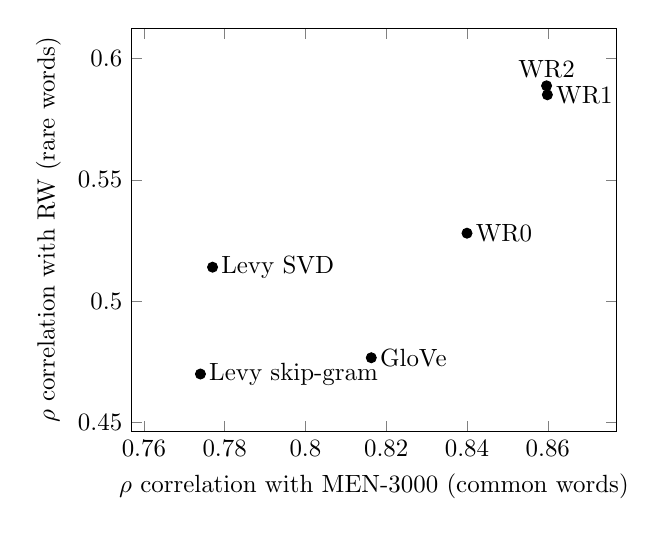
\begin{tikzpicture}[scale=.9]
    \begin{axis}[enlargelimits=0.2, xlabel={$\rho$ correlation with MEN-3000 (common words)}, ylabel={$\rho$ correlation with RW (rare words)}]
        \addplot[
          scatter,mark=*,only marks,nodes near coords,
          point meta=explicit symbolic,
          visualization depends on={value \thisrow{anchor}\as\myanchor},
          every node near coord/.append style={anchor=\myanchor}
        ]
        table[meta=label] {
            x      y     label             anchor
            .777   .514  {Levy SVD}        west
            .774   .470  {Levy skip-gram}  west
            .8163  .4767 {GloVe}           west
            .8400  .5280 {WR0}             west
            .8599  .5850 {WR1}             west
            .8597  .5887 {WR2}             south
        };
    \end{axis}
\end{tikzpicture}
\caption{
    Systems discussed in this paper, plotted according to their $\rho$
    correlation with MEN-3000 and RW.
}
\label{compare-graph}
\end{figure}

% TODO: re-describe for new systems
We have labeled some of the rows of Table~\ref{eval-bigtable} as particular systems
that we would like to compare. System {\bf G} represents a configuration of
GloVe that was evaluated by \newcite{pennington2014glove}. We ran the evaluation
using their provided data, and successfully reproduced their results.

{\bf WR1} and {\bf WR2} are two preferred configurations of our system. {\bf WR1}
applies all the techniques described in this paper as it retrofits with
ConceptNet; {\bf WR2} is the same, but retrofits with a combination of PPDB and
ConceptNet. Both systems perform very well across all word-similarity
evaluations, and it is inconclusive which one is better. We will focus on
system {\bf WR1} for further comparison, because it is simpler.

The numerals in the names {\bf WR1} and {\bf WR2} refer to the number of
additional data sources that were added to the original data using our expanded
version of retrofitting. Another interesting result to compare is {\bf WR0},
the best system that we created without retrofitting anything. This system
simply involves transforming the rows and columns of the existing GloVe 840B
matrix, showing that some of the improvements from this paper can be realized
without introducing any additional data.

It is difficult to compare our system to \newcite{rothe2015} because they only
evaluated on SCWS. Their system can use the full SCWS, because it has a
representation of word contexts, and as such it achieves a higher score than
our system gets on SCWS* without contexts.

Table~\ref{eval-multilingual} shows the performance of these systems on
gold standards that have been translated to other languages, in comparison to
the multilingual results published by \newcite{faruqui2015retrofitting}.
These systems perform well in German, French, and Spanish, even though only
German has a data source designed for it in ConceptNet. French and Spanish terms
are only available because of translations in the English Wiktionary, and
indirect translations via Japanese in JMDict.

\subsection{Comparisons to Other Published Results}

\begin{table*}[t]
\footnotesize
\centering
\begin{tabular}{lrrrrrr}
\toprule
Label   & RW [dev] & RW [test] & RW [all] & MEN [dev] & MEN [test] & MEN [all]\\
\midrule
\bf G   &    .489  &    .448  &    .477  &    .813  &    .816 &    .814 \\
\bf WR0 &    .536  &    .512  &    .528  &    .841  &    .840 &    .841 \\
\bf WR1 &    .587  &    .581  &    .585  &\bf .858  &\bf .860 &\bf .859 \\
\bf WR2 &\bf .591  &\bf .584  &\bf .589  &    .857  &\bf .860 &    .858 \\
\bottomrule
\end{tabular}

\caption{
    A comparison of evaluation results between the ``dev'' datasets that were
    used in development, and the held-out ``test'' datasets, for the systems
    labeled in Table~\ref{eval-bigtable}.
}
\label{eval-dev-test}
\end{table*}

In Table~\ref{compare-others}, we compare our results on the RW and MEN-3000
datasets to the best published results that we know of.
\newcite{levy2015embeddings} present results including an SVD-based method
that scores $\rho = .514$ on the RW evaluation, as well as an implementation
of skip-grams with negative sampling (SGNS), originally introduced by
\newcite{mikolov2013word2vec}. We also compare to the original results from
GloVe's 42-billion-token dataset, and the best MEN-3000 result from
\newcite{faruqui2015retrofitting}.

In relative terms, the performance of our system {\bf WR2} outperforms the best
published RW score (Levy's SVD) by 14.6\%, or 13.6\% if we use our score on only
the test set. Both {\bf WR1} and {\bf WR2} outperform GloVe's result on
MEN-3000 by 5.4\%.

\section{Discussion}

\subsection{Standardizing Term Texts}
% TODO: rewrite to "the importance of text standardization" or something

When we applied ConceptNet's lemmatizer to the labels of GloVe's 840B-token
dataset, we found an unexpected benefit of lemmatization: it caused a very
large performance increase on GloVe 840B even before combining it with any
other data.

When we run our evaluation without lemmatization on the GloVe 42B-token
embeddings, we reproduce the results published in \cite{pennington2014glove}.
This same evaluation, when run on the 840B-token embeddings, produces
surprisingly poor results, implying that some of these rare words appear in
forms that have low-quality embeddings. When we lemmatize the GloVe labels and
combine them using the Zipf estimate, however, the result outperforms the
42B-token embeddings.

It's important to note that we are not changing the evaluation data by using
a lemmatizer; we are only changing the way we look up its embeddings in the
vector space that we are evaluating. For example, if an evaluation requires
similarities for the words ``dry'' and ``dried'' to be ranked differently, or
the words ``polish'' and ``Polish'', the lemmatized system will rank them the
same, and will be penalized in its Spearman correlation.
However, the benefits of lemmatization when evaluating semantic similarity
appear to far outweigh the drawbacks, especially on very large and somewhat
messy data sets such as GloVe 840B.

\subsection{Varying the System}

% TODO: update
In separate experimentation, we found that when we separate ConceptNet into its
component datasets and drop each one in turn, the effects on the evaluation
results are mostly quite small. There is no single dataset that acts as the
``keystone'' without which the system falls apart, but one dataset ---
Wiktionary --- unsurprisingly has a larger effect than the others, because it
is responsible for most of the assertions. Of the 5,631,250 filtered assertions
that come from ConceptNet, 4,244,410 of them are credited to Wiktionary.

Without Wiktionary, the score on RW drops from .587 to .541. However, at the
same time, the MEN-3000 score {\em increases} from .858 to .865. The system
continues to do what it is designed to do without Wiktionary, but there seems to
be a tradeoff in performance on rare words and common words involved.

\subsection{The Limits of Similarity Judgments}

\newcite{bruni2014men} describe a substitute for inter-annotator agreement on
their MEN-3000 dataset:

\begin{quote}
``The Spearman correlation of the two authors is at 0.68, the correlation of their
average ratings with the MEN scores is at 0.84. On the one hand, this high
correlation suggests that MEN contains meaningful semantic ratings. On the
other, it can also be taken as an upper bound on what computational models can
realistically achieve when simulating the human MEN judgments.''
\end{quote}

Our model achieves a MEN score of \scoreMEN{} on the
held-out test data, putting its performance above that upper bound. In many
circumstances, this would be an indication that the model has overfit to the
MEN data. However, we have tried to eliminate the possibility of overfitting.
The MEN data is never used as an input to the system; the same system also
achieves good results on all other data sets; and we did not use or even
look at the held-out data when setting parameters. Strikingly, the evaluation
score on MEN goes {\em up} when the held-out data is evaluated instead.

We postulate instead that similarity evaluations become easier to match
computationally when averaged over the judgments of many people. Notice, for
example, that the two MEN-3000 authors who provided their own ratings
agreed more with the average of the crowd than they did with each other.
If more people's judgments had been averaged in with the authors', perhaps the
correlation would have been even higher. We suspect that, while these results
may be approaching it, the true upper bound of the MEN evaluation is higher than
claimed.

\subsection{Future Work}

% TODO: make these paragraphs flow together?

One aspect of our method that clearly has room for improvement is the fact that
we disregard the labels on relations in ConceptNet, and exclude antonym
relations altogether. There is valuable knowledge there that we might be able
to take into account with a more sophisticated extension of retrofitting, one
that goes beyond simply knowing that particular words should be related, to
handling them differently based on {\em how} they are related.

It was convenient, but not entirely correct, to assume that all of GloVe's data
from the Common Crawl is in English. The Common Crawl is in a wide variety of
languages, just as the Web itself is. In our system, non-English terms are
represented only by links in ConceptNet, but we could have a better starting
point if multilingual terms were represented in the GloVe vectors in the first
place. It could be useful to re-run GloVe in a way that distinguishes languages,
using the metadata on Web pages when available and language-detection heuristics
otherwise.

We believe that the variety of data sources represented in ConceptNet helped to
improve evaluation scores by expanding the domain of the system's knowledge.
There's no reason the improvement needs to stop here. It is quite likely that
there are more sources of ``linked data'' that could be included, or further
standardizations that could be applied to the text to align more data. In
short, these results can probably be surpassed soon. As the second author
observed while running evaluations, ``It seems like every time we do {\em
anything} to the data, the results get better.''

\section{Reproducing These Results}

We aim for these results to be reproducible and reusable by others. The code
that we ran to produce the results in this paper is available in a GitHub
repository at [{\em currently private pending blind review}]. We have tagged
this revision as [{\em TBD}], as we intend to continue to revise and improve the
code afterward. The data files are available at [{\em TBD}], and the README file
in the repository explains how to use {\tt git-annex} to connect the code
with a version-controlled snapshot of the data.

\section*{Acknowledgements}

\begin{CJK*}{UTF8}{min}
\bibliography{wordsim_paper}
\end{CJK*}

\end{document}
